\documentclass[a4paper]{article}

% Packages/Variablen
% #######################
\usepackage[T1]{fontenc}
\usepackage{float}
\usepackage{caption}
\usepackage[utf8]{inputenc} % für Umlaute
\usepackage{ngerman} % Deutsche Rechtschreibung
\usepackage{graphicx}


\title{\begin{center}
		\emph{{\Huge Pflichtenheft}} \\ {\large Kalender}
       \end{center} }
\author{Gruppe 3: Timo Kirfel, Johannes Brautzsch, Alexander Müller}
\date{26.10.2015}

\pdfinfo{ %
  /Title    ()
  /Author   ()
  /Creator  ()
  /Producer ()
  /Subject  ()
  /Keywords ()
}

\begin{document}
  \maketitle
  \newpage

  \tableofcontents % immer 2! mal kompilieren um das inhaltsverz. zu aktualisieren.
		   % beim 1. mal wird das dokument gescannt,
		   % beim 2. mal das inhaltsverzeichnis dazu erstellt.
  \newpage

  \section{Zielbestimmung}
		Es soll eine Kalenderapplikation entwickelt werden, mit welchem Termine übersichtlich und einfach organisiert werden können. Dieses soll für alltägliche Benutzung optimiert und eine grafischen Oberfläche enthält, die intuitiv steuerbar ist.

    \subsection{Musskriterien}
        \begin{itemize}
			\item Grafische Oberfläche in Desktopumgebung
			\item Onlinesynchronisation zu Google
			\item Termine/Gruppentermine verwalten
			\item Mehrbenutzerbedienung
			\item Kontoverwaltung
			\item Verschlüsselung von Benutzerdaten
		\end{itemize}

    \subsection{Wunschkriterien}
        \begin{itemize}
			\item Onlinesynchronisation zu Exchange und Icalendar
			\item Konsolenanbindung
		\end{itemize}

    \subsection{Abgrenzungskriterien}
        \begin{itemize}
	        \item vorerst keine mobile Applikation
	    \end{itemize}

  \section{Produkteinsatz}

    \subsection{Anwedungsbereiche}
			Das Programm soll in einem Desktopsystem realisiert werden.

    \subsection{Zielgruppen}
			Die Anwendung richtet sich an private Nutzer, die keine sonderliche Vorkenntnisse benötigen. Vorgesehen ist die Benutzung von bis zu 5 Personen.

    \subsection{Betriebsbedingungen}
      Für die Benutzer sollen keine langen Wartezeiten entstehen und eine zügige Bedienung möglich sein. Die intuitive Benutzungsweise soll dem Anwender dabei eine Hilfestellung bieten.

  \section{Produktübersicht}
		Das Programm soll plattform unabhängig eingestzt werden können und ist für die Benutzung an einem privaten Heimcomputer konzipiert. Eine gewerbliche Nutzung ist nicht vorgesehen.

  \section{Produktfunktionen}
    \begin{itemize}

			\item[/F010/] Kalanderansicht mit Hilfe einer GUI. Dabei werden Termine grafisch hervorgehoben, sowie und der Titel mit Uhrzeit angezeigt, sofern die aktuelle Ansicht letzteres zulässt.
				\subitem /F011/ Monatsansicht
				\subitem /F012/ Wochenansicht
				\subitem /F013/ Tagesansicht
				\subitem /F014/ Jahresansicht

			\item[/F020/] Der Anwender kann Termine auf zweierlei Arten erstellen:
				\subitem /F021/ Durch Mausklick auf einen Tag/Stunde
				\subitem /F022/ Durch Auswahl „Termin hinzufügen“ in einer Menüleiste.

			\item[/F030/] Die Interaktion in der Kalenderansicht kann sowohl mit dem Mausrad, als auch durch die Cursortasten der Tastatur geschehen.

			\item[/F040/] Am oberen Rand der Benutzungsoberfläche soll eine Menüleiste verfügbar sein, die neben den Kalenderverwaltungsfunktionen die Einstellungen beinhaltet.

			\item[/F110/] Termine kann man für das angemeldete Konto:
			  \subitem /F111/ anlegen
			  \subitem /F112/ löschen
			  \subitem /F113/ ändern

			\item[/F210/] Der Benutzer kann seinen Kalender optional mit einem Onlinekalender synchronisieren, manuell oder automatisch.
			\item[/F220/] Der Anwender kann Benutzer anlegen, die aus Benutzernamen und Kennwort bestehen. Es soll folgende Möglichkeiten geben:
				\subitem /F221/ Benutzer wechseln
				\subitem /F222/ Benutzer löschen
				\subitem /F223/ \textit{Passwort-vergessen}-Funktion
			\item[/F230/] Ein Benutzer kann festlegen, ob und in welchem Intervall sein Kalender einem lokalen Backup abgelegt wird.
			\item[/F240/] Sicheres Beenden des Programms: Schreiboperationen werden dabei zu Ende geführt, und eine notwendige Online-Synchronisierung durchgeführt.
		  \item[/F310/] Optional: Durch die Konsole lassen sich wichtigen Funktionen ausführen, ohne dass die GUI geladen wird. Dazu gehören:
				\subitem /F311/ Termine anlegen, ändern, löschen
			  \subitem /F312/ Benutzer erstellen
			  \subitem /F313/ Synchronisation erzwingen
			  \subitem /F314/ Backup erstellen
			\end{itemize}

  \section{Produktdaten}
	Es sollen folgende Daten persistent gespeichert werden:
	  \subsection{Termine}
	  Termine bestehen aus folgenden Daten (* Pflichtangabe beim Erstellen von Terminen):
        \begin{itemize}
				  \item[/D01/] Titel*
				  \item[/D02/] Datum*, Uhrzeit, Zeitspanne
				  \item[/D03/] Ort
				  \item[/D04/] Besitzer*, Auswahl aus einer Liste vorhandener Benutzer mit der Möglichkeit einen neuen Benutzer anzulegen
				  \item[/D05/] Einzeltermin (Standard) oder Serientyp mit Zyklusangabe
				  \item[/D06/] Beschreibung
				  \item[/D07/] Sichtbarkeit: Privat (Standard) oder Öffentlich
        \end{itemize}
	  \subsection{Benutzerkonto}
		  Zu einem Benutzer gehörigen Informationen:
  		  \begin{itemize}
  		  	\item[/D11/] Benutzername
  		  	\item[/D12/] Passwort (verschlüsselt)
  		  	\item[/D13/] Hinzugefügte Online-Kalender und zugehörige Adressen und Passwörter (verschlüsselt)
  		  	\item[/D14/] Backup- und Synchronisationseinstellungen
  		  		\subitem /D21/ Speicherort/-adresse
  		  		\subitem /D22/ Zeitintervall
		  \end{itemize}


  \section{Produktleistungen}
    \begin{itemize}
	     \item[/L010/] Terminänderungen muss in allen synchronisierten Kalendern übernommen werden. Dies ist abhängig von den Möglichkeiten der Onlinekalender.
	     \item[/L020/] Bei fehlerhaften Eingaben und Daten, darf das Programm nicht abstürzen und es muss dem Benutzer die Möglichkeit zur Änderung der Daten gegeben werden.
			 \item[/L030/] Der Benutzer erhält eine Auflistung aller eingegebenen Fehler.
			 \item[/L040/] Die Datensicherheit wird gewährleistet.
    \end{itemize}

  \section{Qualitätsanforderungen}
    Das Programm darf nicht wegen Benutzungsfehlern abstürzen und soll intuitiv bedienbar sein. Es steht die Benutzungsfreundlichkeit und die Robustheit im Vordergrund. Das Produkt muss keinen industriellen Normen entsprechen.

  \section{Bedienoberfläche}
    \begin{itemize}
		  \item[/B010/] Dem Benutzer wird mittels einer GUI ein Kalender angezeigt, welcher
		  folgende Ansichten unterstützt. Dabei werden Termine grafisch hervorgehoben, sowie und der Titel mit Uhrzeit angezeigt, sofern die aktuelle Ansicht es zulässt.
			  \subitem /B011/ Monatsansicht
			  \subitem /B012/ Wochenansicht
			  \subitem /B013/ Tagesansicht
				\subitem /B014/ Jahresansicht
		  \item[/B020/] Es wird ein grafisches Dialogfeld dargestellt, indem alle Termineinstellungen getroffen werden. Der Anwender kann Termine auf zweierlei Arten erstellen:
			  \subitem /B021/ Durch Mausklick auf einen Tag/Stunde
			  \subitem /B022/ Durch Auswahl „Termin hinzufügen“ in einer Menüleiste
		  \item[/B030/] Die Interaktion in der Kalenderansicht kann sowohl mit dem Mausrad,
		  als auch durch die Cursortasten der Tastatur geschehen.
		  \item[/B040/] Am oberen Rand der Benutzungsoberfläche soll eine Toolbar
		  verfügbar sein, die neben den Kalenderverwaltungsfunktionen auch die
		  Einstellungen darstellt.
			\item[/B050/] Benutzer dürfen nur ihre eigenen privaten Termine und die von ihnen erstellten öffentlichen Termine bearbeiten
			\item[/B050/] Benutzer dürfen öffentliche Termine nur sehen
    \end{itemize}

  \section{Nichtfunktionale Anforderungen}
		\begin{itemize}
			\item Robustheit (Datensicherheit bei Absturz und fehlerhaften Eingaben)
			\item Portablität (Windows, Linux, OSX)
			\item Programmiersprachen: JAVA
			\item Auslieferung: Mitte Januar 2016
			\item Verschlüsselung von lokalen Benutzerdaten
		\end{itemize}

  \section{Technische Produktumgebung}
    \subsection{Software}
	    \begin{itemize}
	    	\item Java Runtime Environment
				\item Betriebssystem: Windows, Linux, OSX
	    \end{itemize}
    \subsection{Hardware}
	    \begin{itemize}
	    	\item Desktop-System mit Bildschirm, Tastatur, Maus
				\item Java Runtime Environment kompatibel
	    \end{itemize}
    \subsection{Orgware}
	    \begin{itemize}
	    	\item keine besonderen Anforderungen
	    \end{itemize}
    \subsection{Entwicklungsschnittstellen}
	    \begin{itemize}
	    	\item Schnittstellen zur Google-Kalender-API, ggf. Ical-Import, Exchange
	    \end{itemize}

  \section{Spezielle Anforderungen an die Entwicklungsumgebung}
    \subsection{Software}
	      \begin{itemize}
	      	\item Editor
					\item Datenbanksystem
	      \end{itemize}
    \subsection{Hardware}
	      \begin{itemize}
	      	\item Desktop-System mit Bildschirm, Tastatur, Maus
	      \end{itemize}
    \subsection{Orgware}
	      \begin{itemize}
					\item Github
	      \end{itemize}
    \subsection{Entwicklungsschnittstellen}
	      \begin{itemize}
	      	\item Google-Kalender-API, ggf. Ical-Import, Exchange
	      \end{itemize}

  \section{Gliederung in Teilprodukte}
    \begin{itemize}
      \item Grafische Oberfläche
		  \item Import von Kalendern
		  \item Synchronisation von Kalendern
    \end{itemize}
  \section{Ergänzungen}
  	\subsection{Fensterdarstellung}
  	\paragraph{}
  	Ein Beispiel für eine Grafische Oberfläche (siehe oben)
  	
  	
	\begin{figure}
		\centering
		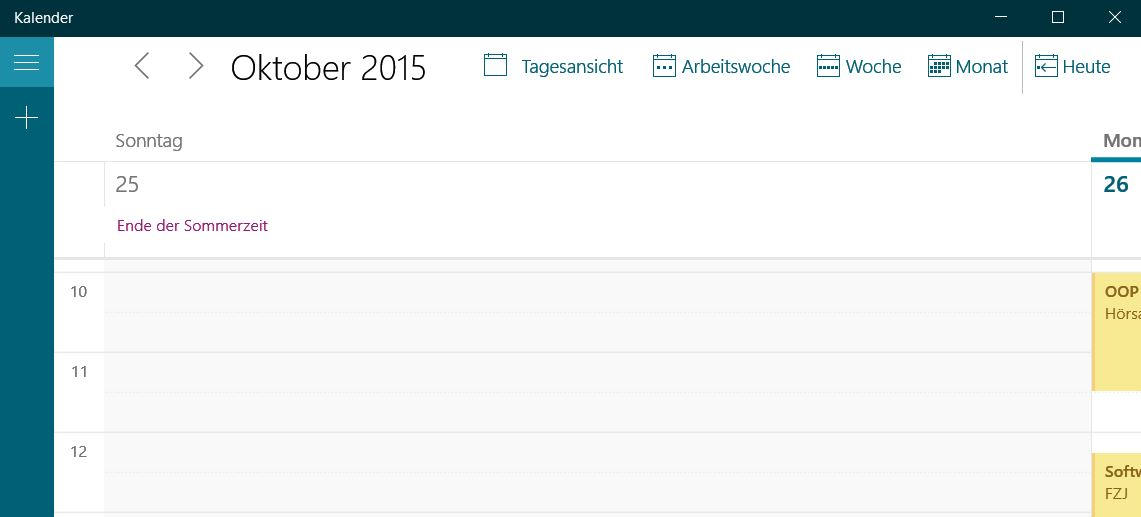
\includegraphics[width=0.9\linewidth]{Fensterdarstellung}
		\caption{}
		\label{Fensterdarstellung}
	\end{figure}


  	
  	\subsection{Andwendungsfalldiagramme}
  	Es sind zwei Anwendungsfälle dargestellt. Der erste Anwendungsfall zeigt einen Akteur, der einen Termin hinzufügt, ändert oder löscht. Die zweite Abbildung wird hier genauer beschrieben: 
  	    \begin{itemize}
  	    	\item Geschaftprozess:
		  	    	Backup anlegen
  	    	\item Akteure:
		  	    	Benutzer
  	    	\item Beschreibung:
		  	    	Der Benutzer hat die Möglichkeit ein Backup seiner Kalender anzulegen.Dies geschiet indem das Programm auf die interne Datenbank zugreift und die geforderten Daten ausliest, verschlüsselt und in eine Datei ausgibt. Des Weiteren kann der Benutzer direkt eine Verbindung zum Online Kalender herstellen und die Kalender auf diesem Weg sichern. Zu dem besteht die Möglichkeit einen Namen für das Backup festzulegen.
  	    \end{itemize}
  	\begin{figure}
		\centering
		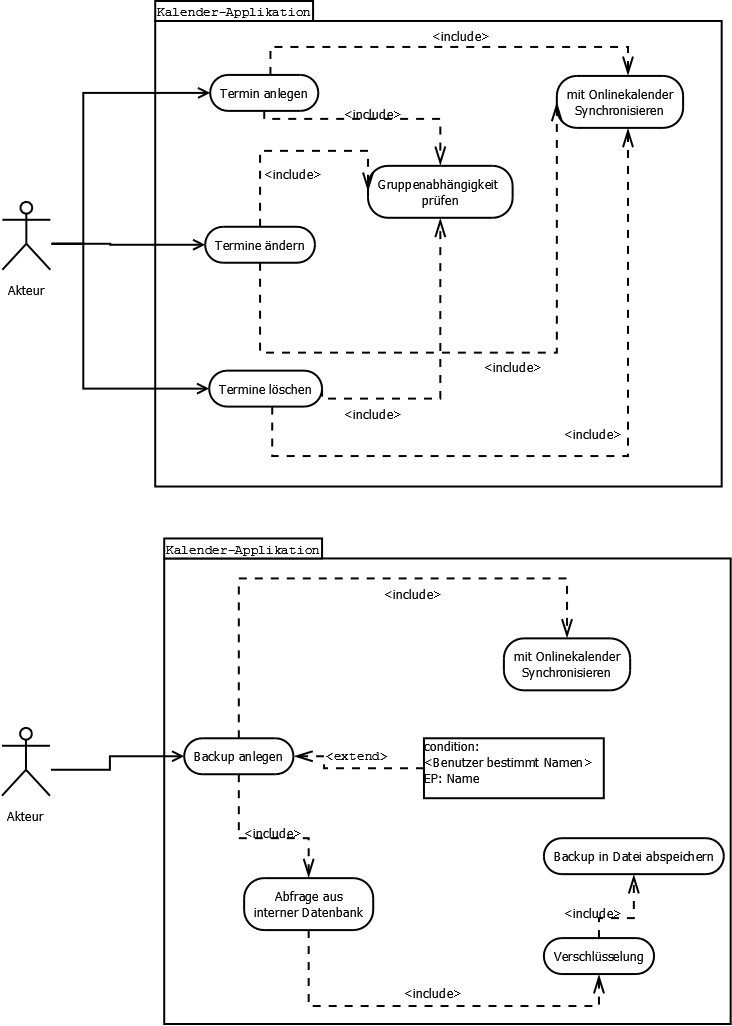
\includegraphics[width=0.9\linewidth]{Anwendungsfalldiagramm.png}
		\caption{}
		\label{Anwendungsfalldiagramm}
	\end{figure}
\end{document}
